\section[A. 聚光灯下]{\myboxi{      \BF{\TT{A}}} 聚光灯下}

\textit{运行时间限制}   5 seconds

\textit{内存使用限制} 1 Gigabyte

\textit{读入文件} \qquad 标准输入

\textit{输出文件} \qquad 标准输出


\begin{quote}
	\textit{当猩红的幕布被缓缓拉开，你便再没有退路。\\
哪怕台下坐着的是漫天神佛，是不可名状的灾厄……\\
只要你还站在台上，这场戏，就必须演到落幕。}
\end{quote}

\subsection{题目描述}

Bean 安置的舞台即将开始美妙的表演 ...

舞台是一个二维欧几里得平面，小人 A 初始站在舞台中心，也即坐标原点 $(0, 0)$. 舞台上方有 $n$ 盏聚光灯，每盏聚光灯会在平面上打出一个以 $(x_i, y_i)$ 为圆心，半径为 $\sqrt{x_i^2 + y_i^2}$ 的圆形光照区，圆形边界也在光照区内，可以发现舞台中心在所有聚光灯的光照区内。

为展现表演的张力，A 希望在表演的移动途中始终在每一盏聚光灯的光照区内，并走到距离舞台中心最远的点。

请帮助 A 求出她在移动轨迹不离开任何一盏聚光灯的光照区的条件下，能走到最远的点到舞台中心的距离。

\subsection{输入格式}

第一行输入一个整数 $T$ ($1 \le T \le 10^5$), 表示测试数据的数量。

每组测试数据第一行输入一个整数 $n$ $(1 \le n \le 10^5)$, 表示聚光灯的数量。

随后 $n$ 行输入两个整数 $x_i$ 和 $y_i$ ($-10^5 \le x_i, y_i \le 10^5$, $(x_i, y_i)$ 不和原点重合)，表示一盏聚光灯的光照区中心。

保证所有测试数据的 $\sum n \le 3 \times 10^5$.

保证单组测试数据中任意两个聚光灯的光照区中心不同，任意三个聚光灯的中心区不共线。

\subsection{输出格式}

对于每组测试数据，输出一行一个实数 $d$ 表示在题述条件下 A 能走到最远的点到舞台中心的距离。

当你输出的实数 $d$ 和标准答案 $ans$ 的绝对误差或相对误差小于 $10^{-6}$ 时，你的答案 $d$ 将会被判为正确。

形式化而言，当 $\frac{|d - ans|}{\max(1, ans)} < 10^{-6}$ 时，你的答案 $d$ 将会被判为正确。

请注意控制你的输出精度总量，不要输出过大的文件，推荐小数点后不要超过 $15$ 位。

\subsection{样例 1}

\begin{minipage}{\linewidth}
	\begin{minipage}[t]{0.49\linewidth}
		\begin{lstlisting}[title=\texttt{standard input}]
2
2
0 1
1 0
4
1 0
0 1
-1 0
0 -1
\end{lstlisting}
	\end{minipage}
	\begin{minipage}[t]{0.49\linewidth}
		\begin{lstlisting}[title=\texttt{standard output}]
1.414213562
0.000000000
\end{lstlisting}
	\end{minipage}
\end{minipage}

\newpage

\subsection{样例 1 解释}


\begin{figure}[htbp]
   \centering
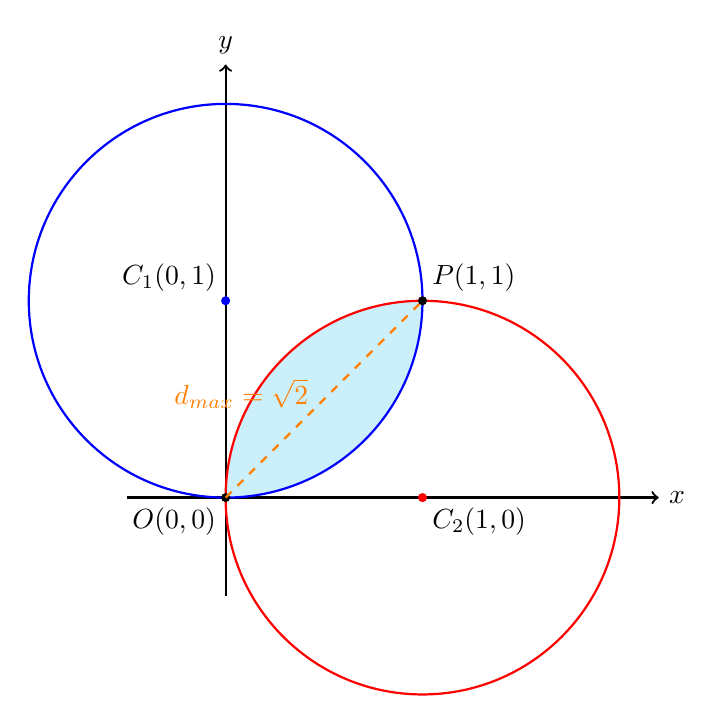
\begin{tikzpicture}[scale=2.5] % 放大比例以提升清晰度
    % 绘制坐标轴
    \draw[->, thick] (-0.5, 0) -- (2.2, 0) node[right] {$x$};
    \draw[->, thick] (0, -0.5) -- (0, 2.2) node[above] {$y$};

    % 填充两个圆的交集（可行域）
    \begin{scope}
        \clip (0,1) circle (1);
        \fill[cyan!20] (1,0) circle (1);
    \end{scope}

    % 绘制第一盏聚光灯的圆 C1(0, 1)
    \draw[blue, thick] (0,1) circle (1);
    \filldraw[blue] (0,1) circle (0.02) node[above left, text=black] {$C_1(0,1)$};

    % 绘制第二盏聚光灯的圆 C2(1, 0)
    \draw[red, thick] (1,0) circle (1);
    \filldraw[red] (1,0) circle (0.02) node[below right, text=black] {$C_2(1,0)$};

    % 标记原点 O(0,0) - 舞台中心
    \filldraw[black] (0,0) circle (0.02) node[below left] {$O(0,0)$};

    % 标记最远点 P(1,1)
    \filldraw[black] (1,1) circle (0.02) node[above right] {$P(1,1)$};

    % 绘制原点到最远点的距离线段（橘色虚线）
    \draw[dashed, thick, orange] (0,0) -- (1,1) node[midway, left, xshift=-2pt, yshift=2pt] {$d_{max} = \sqrt{2}$};

\end{tikzpicture}
\end{figure}

上面的图展示了第 1 组测试数据中的聚光灯光照区，可以发现 A 能走到的最远点为 $(1, 1)$, 答案即为 $d = \sqrt{2}$.

第 2 组测试数据的光照区除了原点外没有别的相交区域了，因此 A 能走到的最远点即为原点 $(0, 0)$，答案为 $0$.

% \subsection{提示}

